\section{Modelli di partenza}

\subsection{Ultralytics}
Ultralytics\cite{40} è un'azienda leader nello sviluppo di soluzioni avanzate di Computer Vision e Deep Learning. Conosciuta principalmente per il suo contributo alla famiglia di modelli YOLO, Ultralytics si distingue per la creazione di strumenti di rilevamento oggetti ad alte prestazioni, ampiamente utilizzati in varie applicazioni industriali e di ricerca. La piattaforma di Ultralytics fornisce modelli pre-addestrati e strumenti di facile utilizzo per l'implementazione rapida di algoritmi di object detection, garantendo prestazioni elevate e scalabilità.

\subsection{Modelli di Ultralytics utilizzati}
Per questo esperimento sono stati scelti i modelli più piccoli per ognuna delle tre tipologie di modello, caratterizzati da una ridotta complessità in termini di numero di parametri da dover addestrare.

I modelli in questione sono:
\begin{itemize}
    \item \textbf{yolov8n}: modello YOLOv8 "nano"\cite{27}
    \item \textbf{yolov8s-world}: modello YOLOv8 "small-world"\cite{30}
    \item \textbf{rtdetr-l}: modello RT-DETR "large"\cite{32}
\end{itemize}

La scelta di questi modelli è stata guidata dalla necessità di avere modelli leggeri e veloci da addestrare, in modo da ottimizzare il processo di sperimentazione e ottenere risultati rapidi senza compromettere significativamente la precisione.

\newpage

\subsection{Valutazione dei modelli}
Per valutare le prestazioni dei modelli ho utilizzato il metodo \texttt{val}\cite{41} fornito da Ultralytics, il quale analizza il comportamento di un determinato modello sul subset specificato nel file di configurazione, fornendo una serie di metriche utili. Il test avviene tramite il seguente script Python, in cui il file di configurazione \texttt{test-config.yaml} specifica al metodo di valutare il modello sul subset di test: 

\begin{figure}[ht]
    \centering
    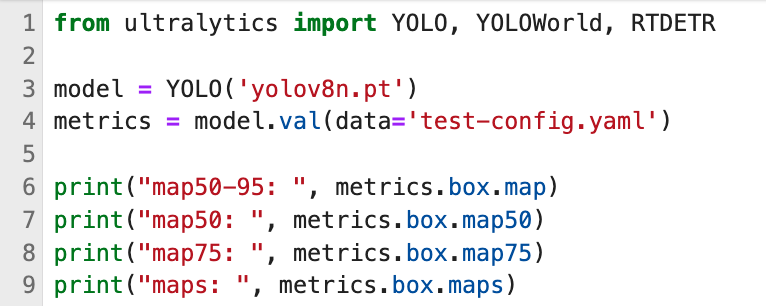
\includegraphics[width=0.5\textwidth]{files/capitoli/4-sperimentazione-risultati/assets/test-script.png}
    \caption{\label{fig:test-script}Script per il testing di 'yolov8n'}
\end{figure}

\subsubsection{Metriche}
Valutare l'efficacia dei modelli di Object Detection richiede l'uso di metriche precise che misurino la capacità del modello di individuare e localizzare correttamente gli oggetti all'interno delle immagini. Le seguenti metriche fondamentali sono essenziali per questa valutazione:

\begin{itemize}
    \item \textbf{Precision}: misura la proporzione di oggetti predetti correttamente rispetto a tutti gli oggetti predetti dal modello.
    \item \textbf{Recall}: misura la proporzione di oggetti veri positivi rilevati correttamente rispetto a tutti gli oggetti veri positivi presenti nel dataset.
    \item \textbf{Average Precision (AP)}: calcola l'area sotto la curva Precision-Recall (PR curve), riflettendo la precisione del modello al variare della soglia di confidenza delle predizioni
    \item \textbf{Intersection over Union (IoU)}: misura la sovrapposizione tra la bounding box predetta e quella ground-truth, ed è calcolato come area dell'intersezione divisa per area dell'unione delle due bounding box.
\end{itemize}

\begin{figure}[ht]
    \centering
    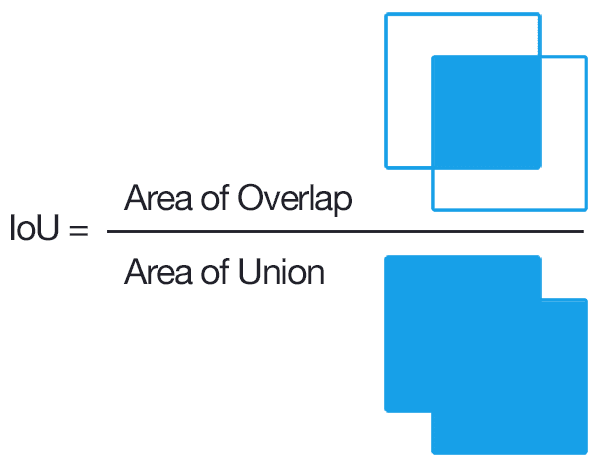
\includegraphics[width=0.4\textwidth]{files/capitoli/4-sperimentazione-risultati/assets/iou.png}
    \caption{\label{fig:iou}Intersection over Union\cite{42}}
\end{figure}

Per valutare più efficacemente le prestazioni dei modelli utilizziamo le metriche di Mean Average Precision (mAP), che rappresentano la media delle Average Precision calcolate per ogni classe:

\begin{itemize}
    \item \textbf{mAP50-95}: media dell'Average Precision (AP) calcolata su diverse soglie di IoU (Intersection over Union), dall'50\% al 95\%
    \item \textbf{mAP50}: media dell'Average Precision (AP) calcolata con IoU al 50\%
    \item \textbf{mAP75}: media dell'Average Precision (AP) calcolata con IoU al 75\%
\end{itemize}

Queste metriche ci forniranno una misura dettagliata delle capacità del modello nel rilevare e localizzare correttamente gli oggetti all'interno delle immagini, considerando diverse soglie di sovrapposizione tra le predizioni del modello e le ground-truth bounding box.

\newpage

\subsection{Test dei modelli non addestrati}

Prima di procedere con l'addestramento dei tre modelli, ho valutato le loro prestazioni iniziali sul dataset filtrato, ottenendo i seguenti risultati:

\begin{figure}[ht]
    \centering
    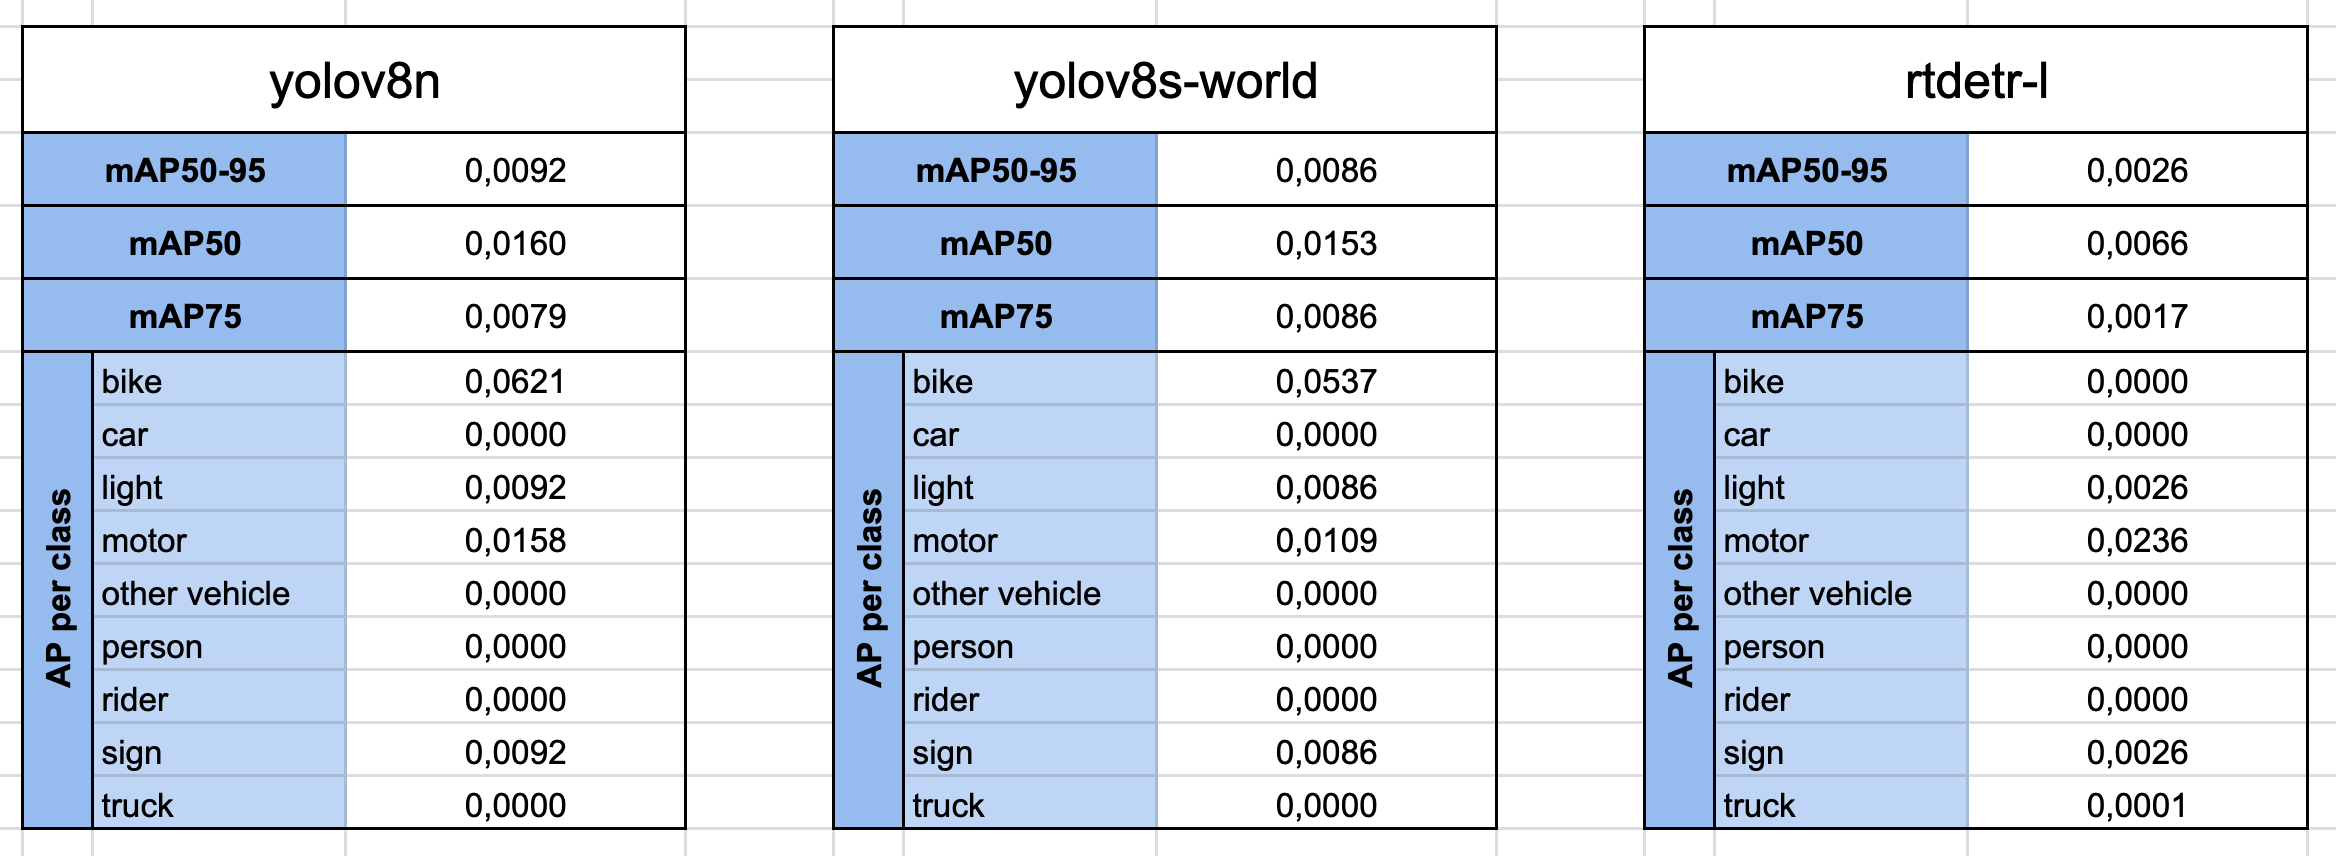
\includegraphics[width=1\textwidth]{files/capitoli/4-sperimentazione-risultati/assets/untrained-metrics.png}
    \caption{\label{fig:untrained-metrics}Risultati test dei modelli non addestrati}
\end{figure}

Possiamo osservare che senza un'ottimizzazione specifica (fine-tuning) sul dataset di immagini termiche, i modelli presentano prestazioni inadeguate nell'Object Detection di questi dati, evidenziando metriche significativamente inferiori rispetto a quelle ottenute sui dataset standard (come COCO) riportate da Ultralytics.

\begin{figure}[ht]
    \centering
    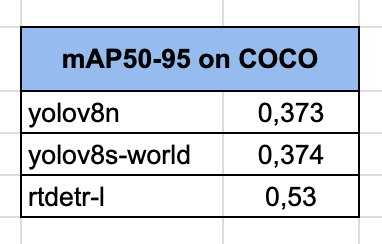
\includegraphics[width=0.3\textwidth]{files/capitoli/4-sperimentazione-risultati/assets/coco-maps.png}
    \caption{\label{fig:coco-maps}mAP50-95 dei modelli su dataset COCO}
\end{figure}

\clearpage

\begin{figure}[ht]
    \centering
    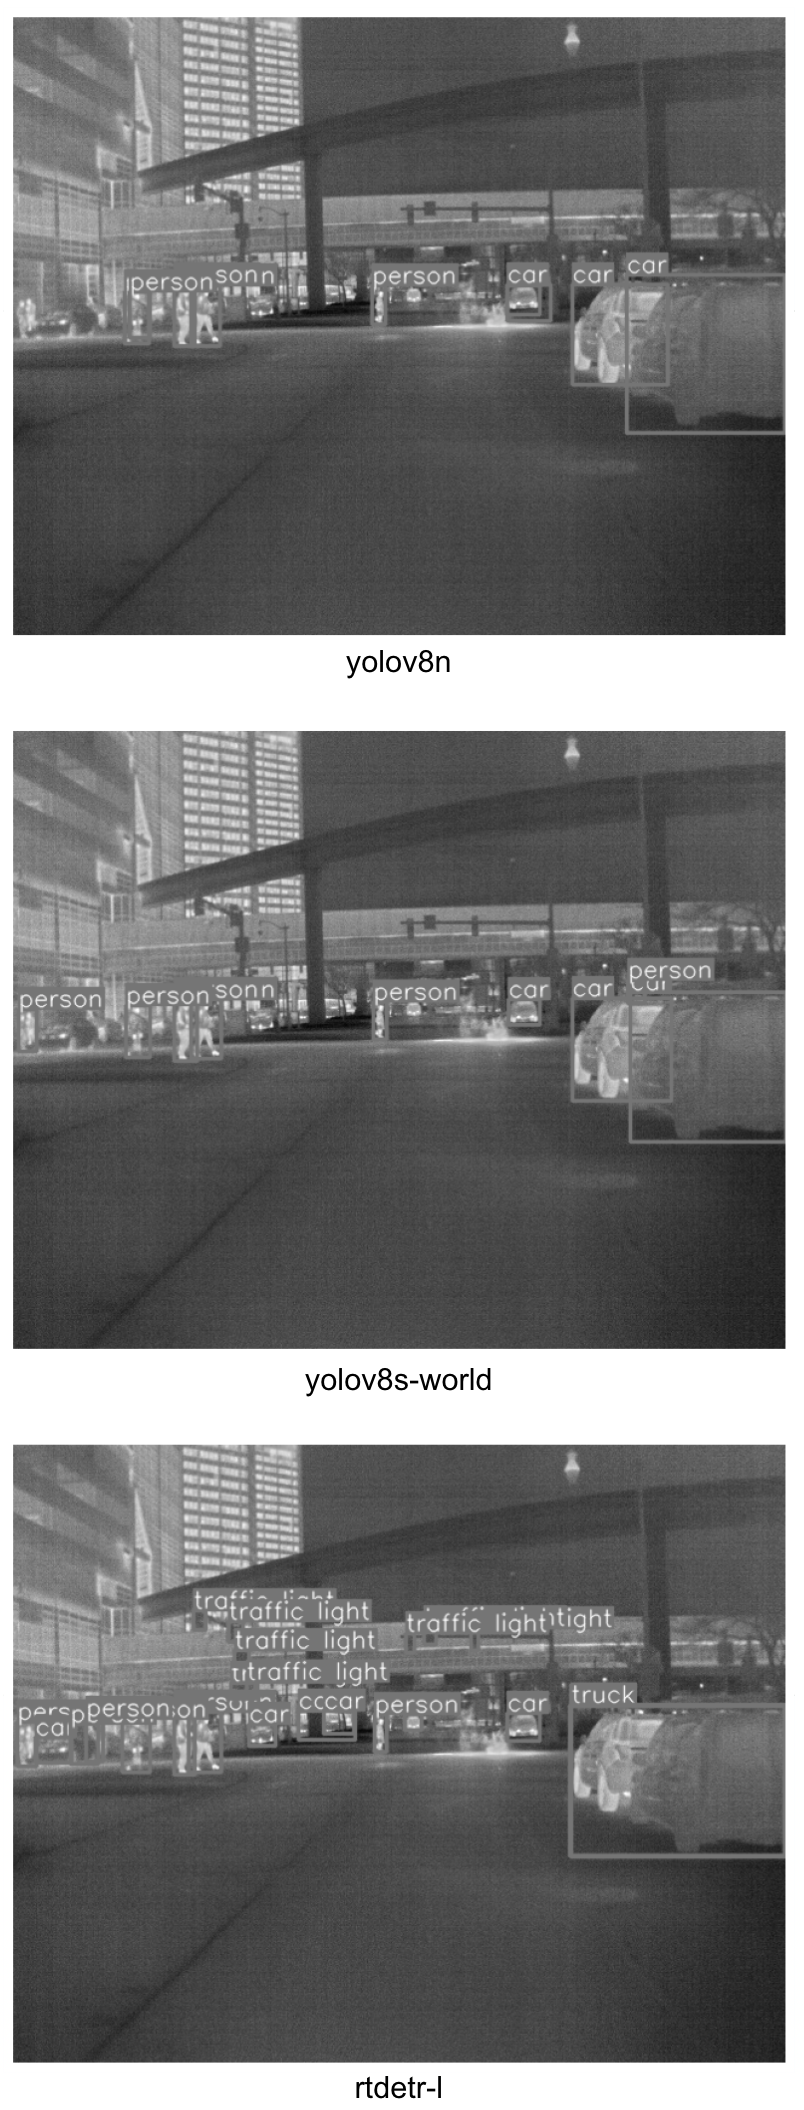
\includegraphics[width=0.6\textwidth]{files/capitoli/4-sperimentazione-risultati/assets/initial-detections.png}
    \caption{\label{fig:initial-detections}Detections effettutate dai modelli non addestrati}
\end{figure}

\clearpage
